\documentclass[11pt,letterpaper]{article}
\usepackage{amsmath}
\usepackage{graphics}
\usepackage{fullpage}
\addtolength{\voffset}{0.5in}

%
%  Cool LaTeX resource:
%   http://en.wikibooks.org/wiki/LaTeX

\begin{document}
\title{Self-improving tutor system}
\author{Brett van de Sande}

% Assignment of blame paper: 
% http://www.public.asu.edu/~kvanlehn/Stringent/PDF/07UM_KVL_KK_etal.pdf
%   my ``opportunity'' equals their ``step''
%   my ``turn'' equals their ``transaction''
%
% Doing reinforcement learning by direct policy search.
% See discussion on p. 17 of:
% http://www.cs.brown.edu/research/pubs/theses/phd/2002/peshkin.pdf


\maketitle

\section*{To do:}

Experimental design:  two conditions: normal Andes and learned
help policy.  For each homework, randomly Divide students into two 
even groups.  Reward for experiment is number of incorrect turns
for each KC while that policy is being enforced.

\section{A model of learning}

For each student and KC, the student has attempted some number of 
{\em steps} that involve that KC.   We will label
steps with $j$.  Usually a given step is associated
with a single user interface object (an equation, vector, etc.)  but
not always, since a student may attempt a particular problem solving
step, delete the object, and later attempt that solution step again.
Each step $j$ corresponds some some number of student-tutor 
{\em transactions}: attempts at constructing the associated object, 
or associated interactions with the Andes help system.  

%Next, we need a model of student learning for a particular KC.
%Since the policies chosen by the random-help version of Andes
%are different for each student,
%we need to determine the point of learning for each student.
For each KC and student, mark each step as ``correct'' if
the student completes the step correctly without any associated errors or 
requests for help; otherwise, the step is marked as ``incorrect.''
%
% From Kurt:
Thus, if each incorrect/correct step is marked with a 0/1, then
a single student's performance on a single KC is a bit string,
{\em exempli gratia} 00101011.

\section{Models of learning}

A number of authors have used a logistic function, 
$\mathrm{logit}(x)=1/\left(1+e^{-x}\right)$, to 
model student learning of a KC.  In that case, we have a two-parameter
model for the probability that the student gets step $j$ correct:
%
\begin{equation}
               P_j^\mathrm{logit} = \mathrm{logit}\left(\beta (j-L)\right)
\end{equation}
%
where $\beta$ is the learning rate and $L$ is 
the the step where the probability of correctness has risen to 50\%.

Alternatively, we can use a function that retains the 
guess $P(G)$ and slip $P(S)$ rates of Corbett and 
Anderson~\cite{anderson}.
The simplest such model is a step-function:
%
\begin{equation}
               P_j^\mathrm{step} = \left\{\begin{array}{cc}
                                       g,& j<L\\
				       1-s,& j\ge L
                                    \end{array}\right. \label{step}
\end{equation}
%
where $g$ is the guess rate, $s$ is the slip rate and 
$L$ is ``the moment of learning,'' the step where the student
first shows mastery of the KC; see Figure~\ref{stepf}.
For a given $L$, we can define an average learning gain,
%
\begin{equation}
     % need actual formula here.
         \Delta_L = 1- \left\langle g+s \right\rangle_L ,
\end{equation}
%
where $\left\langle \cdots \right\rangle_L$ denotes the
expecation value.
\begin{figure}
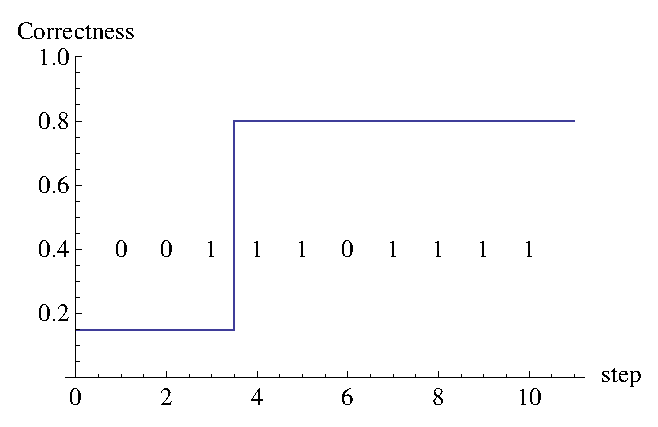
\includegraphics{step.eps}
\caption{The step model with $g=0.15$, $s=0.8$, and $L=4$.}
         \label{stepf}
\end{figure}
%
We can fit $P_j^\mathrm{step} $ to the student data using the
Maximum Likelihood method.
Let $c_i$ \& $w_i$ be the number of correct \& incorrect steps observed
for steps $j<L$ and $c_f$ \& $w_f$ be the number of correct \& incorrect
steps for steps $j\ge L$.  The associated log likelihood for a given $L$ is
%
\begin{equation}
  \mathcal{L}_L  =  \log\left(B_{c_i,w_i}(g)\right) 
                  + \log\left(B_{c_f,w_f}(1-s) \right)  \, ,
		  \label{logLike}
\end{equation}
%
where the guess rate $g$ and slip rate $s$ follow the binomial distribution,
%
\begin{equation}
       B_{a,b}(x) = x^a (1-x)^b\; \frac{(x+b+1)!}{a!\, b!} 
\end{equation}
%
with normalization
%
\begin{equation}
      1=\int_0^1 B_{a,b}(x) \,\mathrm{d}x \; .
\end{equation} 
%
The maximum-likelihood estimators (MLE) for $g$ and $s$ are
%
\begin{eqnarray}
  \hat{g} &=&  \frac{c_i}{c_i+w_i} \, ,\\
  \hat{s} &=&  \frac{w_f}{c_f+w_f} \,  .
\end{eqnarray}
%
Similarly, one can find the maximum-likelihood estimator
for $L$.  However, in some cases, $L$ is not normally
distributed and has a large uncertainty.
So, instead of using the MLE value of $L$ and some
associated error, we will use a multimodel approach~\cite{aic-book}.
We will use a set of models of the form (\ref{step}), 
one for each $L$. Each model has a relative probability given 
by its Akaike weight,  
%
\begin{equation}
                   w_L = \frac{\mathrm{e}^{\mathcal{L}_L-2}}{W}\, ,
\end{equation}
%
with normalization $W$ such that $\sum_L w_L=1$.

%
%  This is not really needed below (remove later)
%
%Finally, we may want to determine whether, in the context
%of the step-function model (\ref{step}), learning has occurred.
%We say that learning has occurred at $L$ if $g<1-s$.
%Since the model is a fit to student data ($c_i$, $w_i$, $c_f$, $w_f$), 
%we can, at best, determine the {\em probability} that learning has occurred. 
%The probability that learning has occurred (for a given L) 
%can be calculated by integrating the Likelihood (see Eqn.~(\ref{logLike})) 
%over the possible slip and guess rates in the region $g+s<1$:
%
%\begin{equation}
%   P(c_i, w_i, c_f, w_f)= \int_0^1 \int_0^{1-g} 
%   B_{c_i,w_i}(g) \, B_{c_f,w_f}(1-s) \,\mathrm{d}g\,\mathrm{d}s
%\end{equation}
%%
%This integral can be solved exactly by repeated integration by parts.


\section{Objective function}

The basic approach for solving this problem, in terms of reinforcement
learning, is called a ``direct policy search.''
For each student, help-giving policy, and KC, we define the objective 
function to be 
%
\begin{subequations}
  \label{objective}
  \begin{align}
  Z =& \sum_L w_L \left\{\sum_{j \in \mathcal{I},\,j<L}  
  % Actually, we use the number of incorrect steps
  % between j and L for the discount factor.
  % need to add this to formula.
       \frac{\gamma^{n(j,L)} \Delta_L}{\left|\sigma_j\right|}
  \sum_{k\in \sigma_j} \left(f(\mathbf{x}_k)-d_k\right))^2 \right.
     \label{before} \\
 % reward for after-learning policy
 % Includes case with no learning as k=0.
  &+\beta \left. \sum_{j \in \mathcal{I},\,j \ge L} \frac{1-\hat{s}}
      {n(L,j_\mathrm{max})\left|\sigma_j\right|}
             \sum_{k\in \sigma_j} \left(f(\mathbf{x}_k)-d_k\right))^2
     \right\}
  \label{after}
  \end{align}
\end{subequations}
%
where $L$ labels different models, each with weight $w_L$;
$\mathcal{I}$ is the set of steps associated
with that student, policy, and KC that were marked ``incorrect.''  
$\sigma_j$ is the set of transactions associated with step $j$,
$f(\mathbf{x}_k)$ is the machine-learned policy associated
with transaction $k$ and
$d_k\in \{0,1\}$ is the
policy actually taken by the random-help version of Andes for that 
transaction.
We have arranged things so that finding an optimal policy 
corresponds to {\em minimizing} $Z$.

The first term (\ref{before}) rewards policies applied directly before
the moment of learning (or step $j=L$ for model $L$).  
These are weighted by the 
average learning gain $\Delta_L = 1-\left\langle g+s\right\rangle_L$ 
predicted by model $L$.
Also, $n(j,L)$ is the number
of incorrect steps $\mathcal{I}$ between $j$ and $L$, 
and $\gamma$ is the ``discount factor''~\cite{ml}. 
A good value for $\gamma \in [0,1]$ must be determined empirically.
In a previous study~\cite{mint}, $\gamma=0.9$ was chosen.
However, in that case, the discount factor was applied transaction-wise in 
a situation where there were many transactions per step.  In our case, 
we apply $\gamma$ step-wise to incorrect steps $\mathcal{I}$, 
suggesting a lower number might be appropriate.

Also, the tutor must have a strategy to apply in the case of slips: 
errors that occur after the student has learned the KC.
The second term (\ref{after}) rewards policies applied after
the KC has been learned.  Since the only available measure of 
effectiveness after the moment of learning is the slip rate $\hat{s}$, 
we look for a policy that maximizes $1-\hat{s}$.  The reward for 
this policy is evenly divided among the $n(L,j_\mathrm{max})$ 
incorrect steps after $L$.
Since our primary objective is to produce learning in the first
place (\ref{before}), we want the contribution of (\ref{after})
to $Z$ to be somewhat smaller.  Thus, we choose $\beta$ numerically 
such that the contribution of (\ref{after}) is somewhat smaller than 
the contribution of (\ref{before}).

The machine learning algorithm finds a function $f$ that acts on
the set of states $\left\{\mathbf{x}_k\right\}$ that minimizes
the objective function $Z$ summed overs students and KC's.  
Since our policies are binary-valued
and many of our features are well ordered (times, counts of transactions,
{\em et cetera}), it is natural to define $f$ in terms of a 
linear classifier.  Thus
%
\begin{equation}
              f(\mathbf{x}_k) = \left\{\begin{array}{cc}
		1,& \mathbf{a}\cdot \mathbf{x}_k <b \\
                0, & \mathbf{a}\cdot \mathbf{x}_k \ge b
		\end{array} \right.
\end{equation}
%
That is, $\mathbf{a}$ and $b$ define a hyperplane in feature
space.  All states on one side of the plane are given policy 0
and states on the other side have policy 1.
Numerically, we find $\mathbf{a}$ and $b$ that minimizes $Z$
summed over students and KC's.

\section{Feature space}

The student state at any given time is described by a list of
features.   Since the machine learned policy is to act on this list of
features, they must be computable in real time.  This is can be a
challenge in tutor system with a free-form interface like  Andes:
there is not always a way to determine, in real time, what a student was
attempting when they make an entry and get it wrong, even if the attempt
is examined by an expert human tutor.  Andes has a
number of error handlers that do make such a determination, but they 
apply only for certain well-known errors.

For determining which features to select, we used Min Chi's thesis
as a starting point~\cite{mint}, although she was doing this for a
rather different kind of tutor system.  The following items were
chosen mostly for convenience, and they avoided issues with determing
the KC associated with an entry.
%
\begin{description}

\item[logSessionTime] Log of number of seconds since start of current
  session.  This is a measure of student fatigue.

\item[fracSessionFlounderTime] Flounder time is the time spent between 
incorrect (object turns red) transactions, with no intervening correct 
(object turns green) transactions. 
 {\em fracSessionFlounderTime} is the total flounder
time for the current session over total session time.

\item[logNowRedTrans] Log of number of transactions since last
  correct (object turns green) transaction.

\item[logNowRedTime] Log of number of seconds since last
  correct (object turns green) transaction.

\item[logNowIdleTime] Log of number of seconds since last transaction.

\item[sessionCorrect] Number of objects in current session that have
  been  been marked  correct.

\item[sessionIncorrect] Number of transactions in current session where 
   object has been marked  incorrect.

\item[sessionHelp] Number of help requests in current session.

\item[fracSessionCorrect] $\mbox{sessionCorrect}/\left(\mbox{sessionCorrect}+\mbox{sessionIncorrect}+\mbox{sessionHelp}\right)$.

\end{description}
%
We have taken the logarithm of quantities where the student data
for that quantity ranges over several orders of magnitude.

On the Andes help server, the state for a given transaction 
is determined before the student action itself is analyzed,
in order that the help policy for that transaction can be set.  
Thus the state can only depend correct/incorrect (or floundering) 
information from previous transactions. 

\begin{thebibliography}{9}

\bibitem{anderson} 
  Corbett, A.\ T., Anderson, J.\ R. Knowledge Tracing:  Modeling 
the Acquisition of Procedural Knowledge.  \emph{User Modeling and
 User-Adapted Interaction}, 1995, 4, 253--278.

\bibitem{beckchang}
  Beck, J.\ E., Chang, K.-m.\ Identifiability: A Fundamental Problem of
  Student Modeling.
  \emph{Proceedings of the $11^{th}$ International Conference on User 
    Modeling}, 2007.

\bibitem{aic-book}Burnham, K.~P., and Anderson, D.~R. \emph{Model
  Selection and Multimodel Inference: A Practical
  Information-Theoretic Approach}, 2nd ed. Springer-Verlag. 2002.

%\bibitem{aha}Kurt and Kasia moment of learning paper.

\bibitem{ml}Discount factor citation.

\bibitem{mint}Min's Thesis (or publication?)

\bibitem{linear}Linear classifier Ref. 
     http://en.wikipedia.org/wiki/Linear\_classifier

\end{thebibliography}




\end{document}